% Beamtime April 2015
Further experiments were carried out to increase the cleanlyness of the h-BN on the polycrystalline copper foil. To reduce the amount of elements coming from the body of the foil it is repeatedly sputtered and annealed to temperatures as high as \SI{800}{\degreeCelsius}. This may have also an improving influence on the grainsize and amount of corrugation. Several attempts have been made which are described in summary below.
%%%%%%%%%%%%%%%%%%%%%%%%%%%%%%%%%%%%%%%%%%%%%%%%%%%%%%%%%%%%%%%%%%%%%%%%%%%%%%%%%%%%%%%%%%
\begin{itemize}
 \item After cleaning, the sample is inverstigated in STM. The foil shows a inhommogenous topography, with parts of the sample showing very flat regions (figure \ref{fig:30-31.03}) while others still remain heavily corrugated.
\end{itemize}
% -----------BILDER ---- DISKUSSION: 30.03/31.03
\begin{figure}[h!]
 \centering
 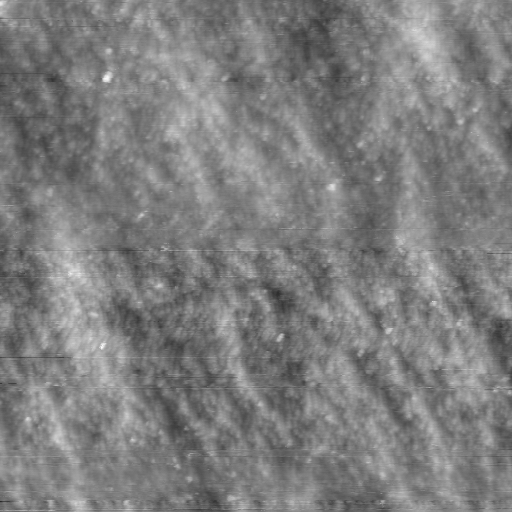
\includegraphics[width=0.5\textwidth]{./images/F150331-124839.jpg}
 \caption{Cu-foil after repeated sputtering and annealing cycles. Roughness $\approx \SI{100}{\pico\meter}$. Compare figure \ref{fig:cu-foil-clean}.}
 \label{fig:30-31.03}
\end{figure}
%%%%%%%%%%%%%%%%%%%%%%%%%%%%%%%%%%%%%%%%%%%%%%%%%%%%%%%%%%%%%%%%%%%%%%%%%%%%%%%%%%%%%%%%%%
\begin{itemize}
 \item Before dosage the sample was kept at \SI{800}{\degreeCelsius} for another 10 minutes.
Borazine was dosed for 5 minutes with a pressure of \SI{1e-7}{\milli \bar} with the sample kept at temperatures of \SI{850}{\degreeCelsius}. Afterwards the sample was kept at this temperature for another minute.
\end{itemize}
%  -----------BILDER ---- DISKUSSION: 15.04
% \begin{figure}
%  \centering
%  \includegraphics[width=0.5\textwidth]{./images/}
%  \caption{}
%  \label{fig:15.04}
% \end{figure}
%%%%%%%%%%%%%%%%%%%%%%%%%%%%%%%%%%%%%%%%%%%%%%%%%%%%%%%%%%%%%%%%%%%%%%%%%%%%%%%%%%%%%%%%%%
\begin{itemize}
 \item The sample was sputtered and annealed several times to temperatures of \SI{800}{\degreeCelsius}. Before the dosage it was held 5 minutes at \SI{750}{\degreeCelsius}. Borazine was dosed with the same pressure as before (\SI{1e-7}{\milli \bar}) but for 1min and at a lower temperature of \SI{750}{\degreeCelsius}. After the preparation the sample was kept at \SI{750}{\degreeCelsius} for another 1 minute. It was cooled down slowly (shown in figure \ref{fig:16.04}.
\end{itemize}

\begin{figure}
 \centering
 \includegraphics[width=0.5\textwidth]{./images/F150416-192611.jpg}
 \caption{STM image after 4\,L of borazine dosage on a \SI{800}{\degreeCelsius} hot Cu-foil surface. A little h-BN island can be seen on a largely uncovered copper foil background (lower right).}
 \label{fig:16.04}
\end{figure}
% -----------BILDER ---- DISKUSSION: 16.04
% %%%%%%%%%%%%%%%%%%%%%%%%%%%%%%%%%%%%%%%%% false preparation %%%%%%%%%%%%%%%%%%%%%%%%%%%%%%
% The next preparation step was started with an intense cleaning step of the copper foil. It was sputtered and annealed to \SI{750}{\degreeCelsius} twice and then kept at \SI{830}{\degreeCelsius} for 2 hours. After this it was sputtered and annealed to \SI{750}{\degreeCelsius} for 1 minute before the borazine was dosed. Unfortunatly the exact amount of borazine could not be determined, the pressure increased to \SI{1e-4}{\milli \bar} for a very short time, so that the dosage was interrupted well below 1 minute. It was again hold at the temperature for another minute and was cooled down very slow (\SIrange{1}{3}{\kelvin \per \second}). The mass spectrum taken after deposition shows the highest peak not where the intact borazine molecule is located but somewhere to lower masses. This indicates that the borazine has decomposed.
% 
% -----------BILDER ---- DISKUSSION: 17.04
%%%%%%%%%%%%%%%%%%%%%%%%%%%%%%%%%%%%%%%%%%%%%%%%%%%%%%%%%%%%%%%%%%%%%%%%%%%%%%%%%%%%%%%%%%
\begin{itemize}
 \item The foil was sputtered and annealed 4 times with temperatures of \SI{800}{\degreeCelsius}. Borazine was dosed at \SI{2e-7}{\milli \bar} for \SI{2.5}{\minute}. The sample was kept at this temperature for another 5 minutes after dosing. The sample was cooled down slowly. Figure \ref{fig:15.04} shows some of the grown islands. The copper surface changes upon h-BN growth and the terrace width increases below the h-BN flakes. The typical facetting of the surface vanishes or can at least not be depicted because of the overgrowing h-BN (figure \ref{fig:23.04}). Due to nearby tip formings, the right side of the image is decorated with adsorbats, most likely from the tip itself - they appear as bright white spots in the image.
\end{itemize}
% -----------BILDER ---- DISKUSSION: 21.04
\begin{figure}
 \centering
 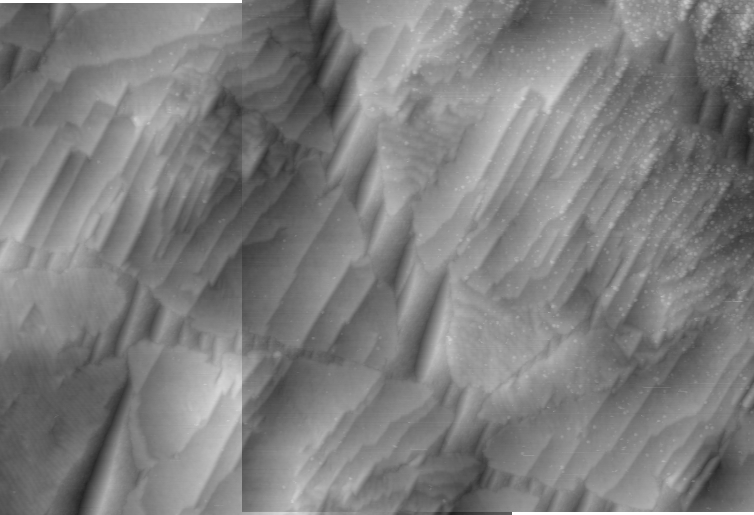
\includegraphics[width=\textwidth]{./images/150423-1008-1027}
 \caption{STM image of 22\,L boarazine dosed on a \SI{800}{\degreeCelsius} hot copper-foil surface. Serveral large islands can be seen that grow over Cu-foil step edges. Defiled right hand side of the image due to nearby tip forming. Overlay of two images. Image height: \SI{295}{\nm}}
\end{figure}

\begin{figure}
 \centering
 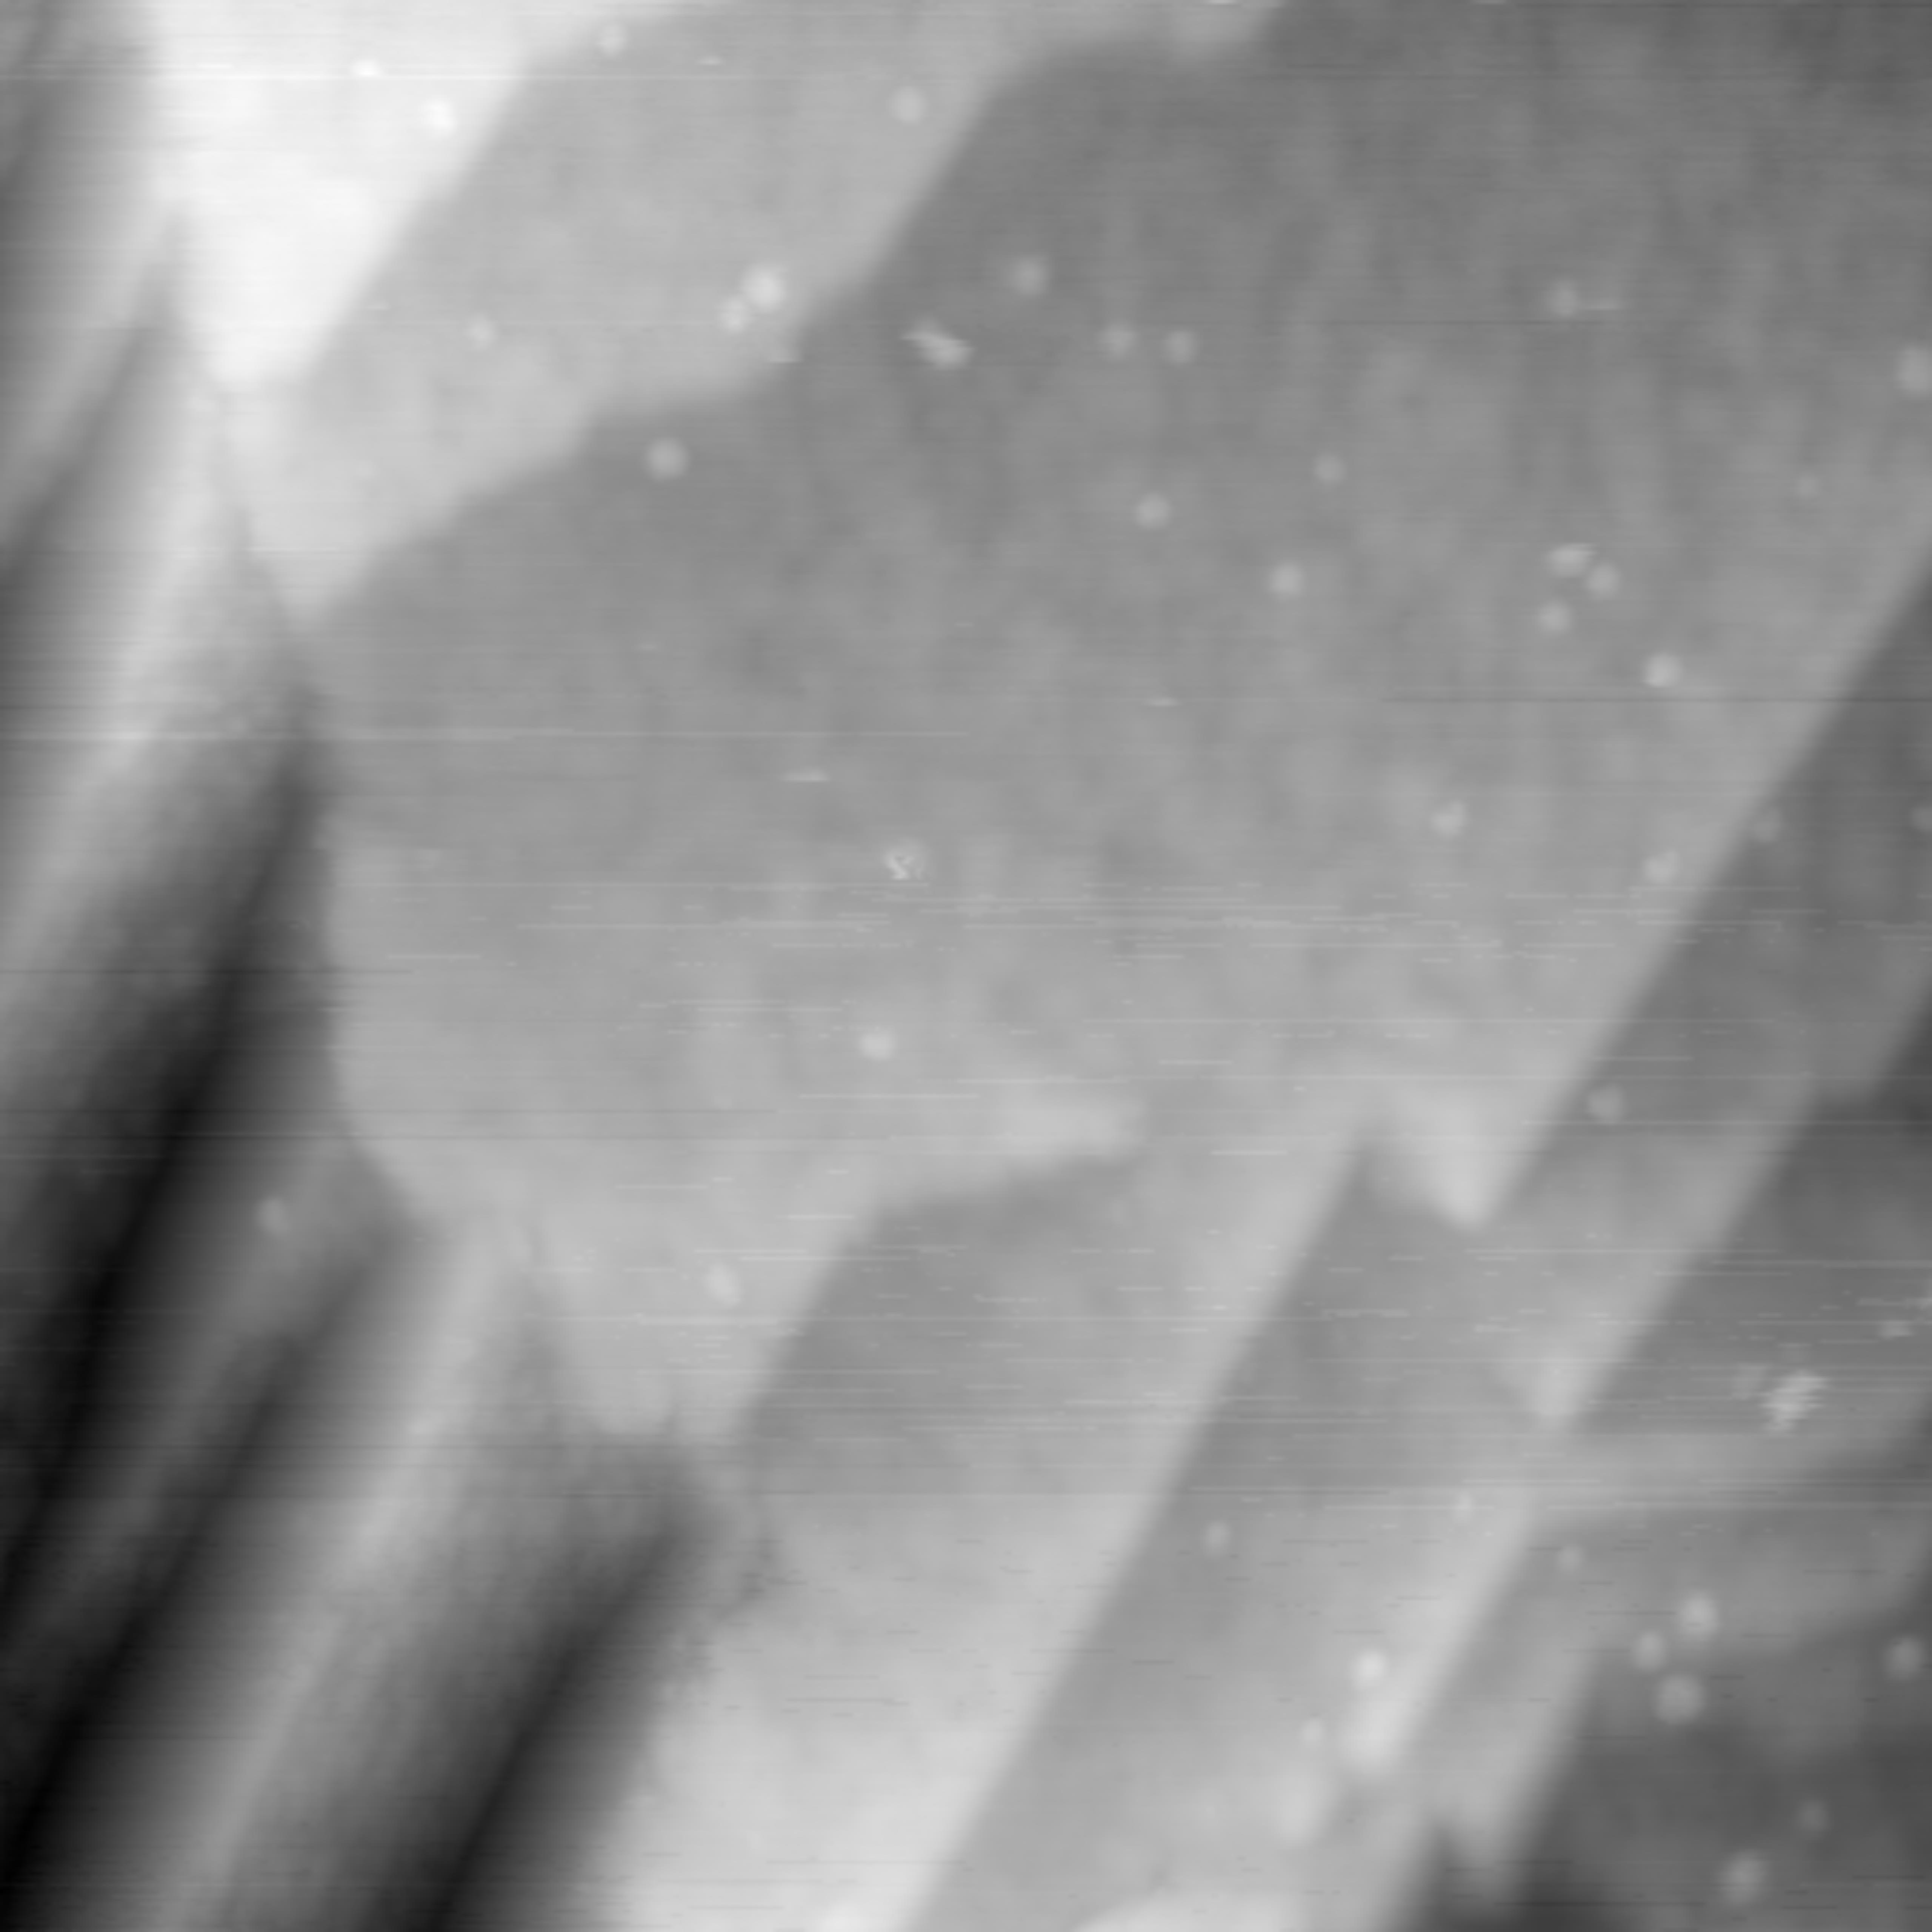
\includegraphics[width=0.5\textwidth]{./images/F150423-114214.jpg}
 \caption{STM image of island that overgrows Cu-foil facets.}
 \label{fig:23.04}
\end{figure}

%%%%%%%%%%%%%%%%%%%%%%%%%%%%%%%%%%%%%%%%%%%%%%%%%%%%%%%%%%%%%%%%%%%%%%%%%%%%%%%%%%%%%%%%%%
points to point out:
\begin{itemize}
 \item Look at Messzeit-April.ppt power point presentation
 \item Stufenh\"ohe
 \item Beschaffenheit der stufen/facetts
 \item Wechselwirkung BN-Wachstum und Facettenbildung
\end{itemize}